\section{Clustering Summary}

Three methods based on the hierarchical clustering are proposed to solve the authorship clustering task.

The first is based on the mean Silhouette score to find the best clustering at each step of the hierarchical clustering.
The second uses an author links distribution model to find the best step to stop the hierarchical clustering.
And the last is based on a logistic regression model to estimate the true link probability for new rank lists.
These methods are summarized in the schema in Figure~\ref{fig:schema-clustering}.

Table~\ref{tab:clustering_evaluation_summary} contains a evaluation summary of the proposed method.
The evaluation use the $B^3_{F_1}$ score and the $r_{diff}$ metrics.

Each method produce similar results, but the distribution-based clustering with complete linkage give the best results, $B^3_{F_1} = 0.82$.
The Silhouette-based methods and the regression-based method produce slightly less accurate results.
The non-tweak Silhouette-based model give the least accurate results.

The complete linkage and average linkage criterion give the best results.
Though the average linkage criterion have better results with three out of the four models, the distribution based model with the complete linkage give the best results across the board.
It reaches an $B^3_{F_1} = 0.82$.
Since the single linkage criterion produce weak results for every model, this criterion is left aside for the next experiments.

Three models give the best approximation of the number of clusters with $r_{diff} = 0.06$:
The Silhouette-based model with average linkage or complete linkage, and the distribution-based model with average linkage.
These models are close to find the right number of clusters almost every time.

We compare the models with the upper bound.
The upper bound is the best clustering achievable using the same rank lists as for the model evaluation.
The upper bound is found by evaluating the clusters $B^3_{F_1}$ score at each step of the hierarchical clustering.
The step with the best metrics are kept for each rank list.
The values exposed in this table are the average metrics of each \textit{best clustering} for the rank lists.

Overall, the results are close to the upper bound.
The best $B^{3}_{F_1}$ achieved with each model is $8-15\%$ worse than the upper bound.

\begin{figure*}[!t]
  \centering
  \caption{Clustering methods schema}
  \label{fig:schema-clustering}
  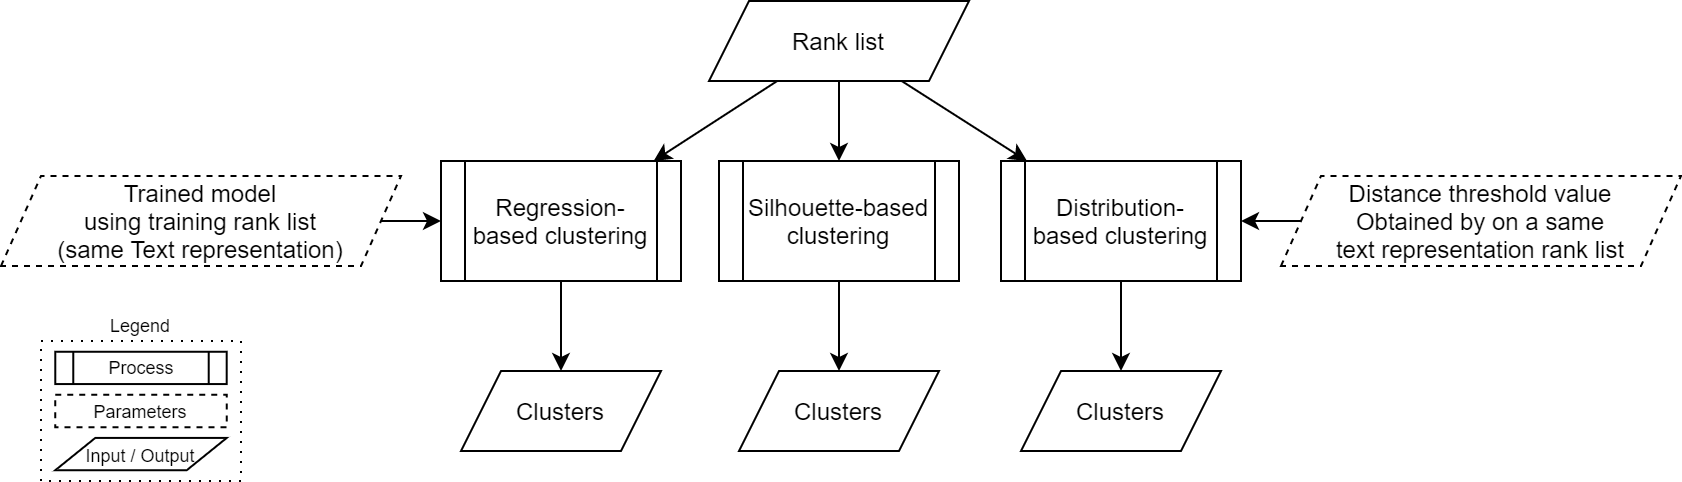
\includegraphics[width=1\linewidth]{img/schema-clustering.png}
\end{figure*}

\begin{table*}[!t]
  \centering
  \caption{Mean retained rank lists $B^{3}_{F_1}$/$r_{diff}$ for each clustering method}
  \label{tab:clustering_evaluation_summary}
  \begin{tabular}{l c c c}
    \toprule
                                       & \multicolumn{3}{c}{Linkage criterion} \\
    Clustering method                  & Single         & Average            & Complete \\
    \midrule
    Silhouette-based ($\alpha = 0$)    & 0.74/0.22      & \textbf{0.76/0.17} & 0.75/0.17 \\
    Silhouette-based ($\alpha = -0.2$) & 0.79/0.08      & \textbf{0.81/0.06} & 0.80/0.06 \\
    Distribution-based                 & 0.22/0.16      & 0.76/0.06          & \textbf{0.82/0.07} \\
    Regression-based                   & 0.64/0.10      & \textbf{0.80/0.13} & 0.74/0.19 \\
    \midrule
    \textit{Rank lists upper bound}    & \textit{0.83/0.00} & \textit{0.88/0.00} & \textit{0.87/0.00} \\
    \bottomrule
  \end{tabular}

  \vspace{0.2cm}
  \textbf{In bold}: The linkage criterion with the largest $B^{3}_{F_1}$ for each clustering method.
\end{table*}
